\documentclass[oneside,spanish]{amsart}
\usepackage[T1]{fontenc} % Tipo de fuente
\usepackage[utf8]{inputenc} % Archivo UTF-8
\usepackage[a4paper]{geometry}
\geometry{verbose,tmargin=2cm,bmargin=2cm,lmargin=3cm,rmargin=2.5cm} % Tamaño
\usepackage{amsthm} 
%\usepackage{amsaddr} % Para modificar la posición de address
\usepackage[spanish]{babel} % Idioma español
\usepackage[backend=biber,style=alphabetic,natbib,maxalphanames=1]{biblatex} % Compilar bibliografía con BibLaTeX (no BibTeX)
\usepackage[shortlabels]{enumitem} % Mejora el entorno enumerate
\usepackage{graphicx} % Colocar imágenes
\usepackage[hidelinks]{hyperref} % Vínculos y referencias interactivas
\usepackage[skip=3pt]{caption} % Permite modificar el espacio entre el caption y la imagen
\usepackage{multicol} % Entornos de múltiples columnas

%-------------------------------------------------------------------------
% Configuraciones iniciales
\makeatletter
%Numeración
\numberwithin{equation}{section}
\numberwithin{figure}{section}
\newlength{\lyxlabelwidth}      % Longitud auxiliar
\makeatother
%-------------------------------------------------------------------------

%-------------------------------------------------------------------------
% Bibliografía
\defbibheading{bibliography}[\refname]{}
\addbibresource{refs-tall03.bib}

\renewcommand*{\labelalphaothers}{}

\DeclareLabelalphaTemplate{
  \labelelement{
    \field[final]{shorthand}
    \field{labelname}
    \field{label}
  }
  \labelelement{
    \literal{,\addhighpenspace}
  }
  \labelelement{
    \field{year}
  }
}
%-------------------------------------------------------------------------

%-------------------------------------------------------------------------
% Otras configuraciones
%\pagestyle{plain} % Para que el encabezado esté vacío
\addto\captionsspanish{\renewcommand{\tablename}{Tabla}}
\addto\captionsspanish{\renewcommand{\figurename}{Figura}}

\theoremstyle{definition}
\newtheorem{problema}{\normalfont PROBLEMA}
%-------------------------------------------------------------------------

\usepackage{fancyhdr}
\pagestyle{fancy}
\fancyhf{} % sets both header and footer to nothing
\renewcommand{\headrulewidth}{0pt}
\fancyhead[C]{\scriptsize\MakeUppercase\shorttitle}

%-------------------------------------------------------------------------

% Y acá comienza el documento

\begin{document}
	
%-------------------------------------------------------------------------
% Datos del artículo
\title{Funciones polinómicas y GeoGebra\vspace{-2ex}}
\author[1]{Noemí Paola Paz\textsuperscript{1}}
\author[2]{Josefina Lávaque Fuentes}
\author[3]{Cintia Celeste Solaliga}
\author[4]{Mariel Fadon}
\email[corresponding author]{\textsuperscript{1}paolapaz32@gmail.com}
%-------------------------------------------------------------------------

\begin{abstract}
	  La propuesta de taller que estamos presentando surgió a raíz del análisis sobre la problemática de la enseñanza de polinomios y funciones polinómicas en las aulas de la escuela secundaria. La misma retoma una secuencia puesta en aula cuya intencionalidad fue poner a los estudiantes en un rol protagonista de las clases y productores de conocimiento, permitiendo explorar a partir del uso del GeoGebra asuntos matemáticos relacionados a la temática. Además consideramos que la herramienta habilita a nuevas discusiones y modos de validación.
\end{abstract}

\maketitle
\thispagestyle{empty}

\section{Contenidos}

Las funciones como objeto matemático y como objeto de enseñanza. Registro algebraico. Lectura de una fórmula. Relación gráfico-fórmula en funciones polinómicas. El vínculo entre las funciones polinómicas y los polinomios. Una mirada sobre expresiones factorizadas de una función polinómica como un producto de otras funciones polinómicas. Nuevos aspectos del trabajo matemático en entornos informáticos. El papel del GeoGebra en la exploración, producción de conjeturas, anticipación y validación.

\section{Requisitos Previos}

Función lineal. Propiedades y características. Función cuadrática. Características. Uso del GeoGebra.

\section{Objetivos}

Reflexionar sobre el potencial didáctico de estudiar lo funcional por medio de la noción de variación y el rol del proceso de modelización en dicho estudio.

Analizar la potencia y los límites de cada registro de representación semiótica en relación al conocimiento sobre las funciones que se puede construir a partir de ellos.

Concebir nuevas significaciones y relaciones que se pueden producir a partir de la las transformaciones de un registro a otro y la coordinación entre ellos.

Profundizar la reflexión sobre el rol docente en el aula de matemática promoviendo y sosteniendo espacios de discusión y producción de conocimiento.

\section{Actividades}

\subsection{Actividades Previas}

En el espacio destinado para el taller se habilitará la siguiente consigna.

\paragraph{Actividad del taller:} 
Considerando los problemas 1, 2 y 3:
\begin{itemize}[-]
	\item Anticipar posibles resoluciones de los chicos y las chicas para cada ítem. 
	\item Estudiar qué estrategias podrían estar más disponibles dependiendo de los números propuestos en cada caso. ¿Dónde puede haber dificultades en la tarea y cuáles pueden ser?
	\item Les pedimos que armen un escrito con la resolución de esta consigna posible de ser compartido en el sincrónico. 
\end{itemize}

\begin{problema}\label{prob:1}

Sean $f(x)$ y $g(x)$ dos funciones lineales. Definimos la función $h(x)$ de la siguiente manera: para cada valor de $x$, $h(x) = f(x) \cdot g(x)$. A partir de los gráficos de $f(x)$ y de $g(x)$ que se dan a continuación, (figura \ref{fig:imagen1}),

\begin{figure}[h]
	\centering
	\caption{}
	\label{fig:imagen1}
	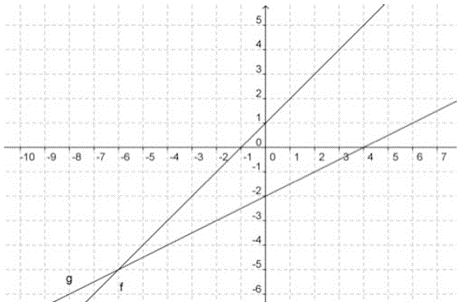
\includegraphics[width=0.7\linewidth]{Anexos-03/Imagen1}
\end{figure}

\begin{enumerate}[a.]
	\item Calculen el valor de h(x) en cada caso:
	\begin{multicols}{4}
		\begin{enumerate}[i.]
			\item $h(0)=$
			\item $h(2)=$
			\item $h(6)=$
			\item $h(3)=$
			\item $h(-2)=$
			\item $h(4)=$
			\item $h(-8)=$
			\item $h(4,5)=$
		\end{enumerate}
	\end{multicols}
	
	\break
	
	\item Decidan si h(x) es negativa, positiva o cero:
	\begin{multicols}{5}
		\begin{enumerate}[i.]
			\item $h(-10)$
			\item $h(-20)$
			\item $h(-1)$
			\item $h(5)$
			\item $h(-2,5)$
		\end{enumerate}
	\end{multicols}
	
	\item Propongan un gráfico aproximado de $h(x)$.
\end{enumerate}
\end{problema}

\begin{problema}\label{prob:2}

En el siguiente sistema de coordenadas se dan las gráficas de f(x) y g(x), ambas funciones lineales. (Figura \ref{fig:imagen2})

\begin{figure}[h]
	\centering
	\caption{}
	\label{fig:imagen2}
	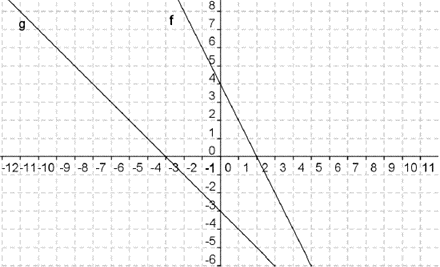
\includegraphics[width=0.7\linewidth]{Anexos-03/Imagen2}
\end{figure}

Definimos: $h(x) = f(x) \cdot g(x)$.

\begin{enumerate}[a.]
	\item Encuentren por lo menos 3 puntos que pertenezcan al gráfico de $h(x)$. Propongan argumentos para fundamentar la respuesta.
	\item Establezcan el conjunto de valores de $x$ para los cuales la función $h(x)$ es positiva, negativa o cero.
	\item Tracen un gráfico aproximado de $h(x)$.
\end{enumerate}
\end{problema}

\begin{problema}\label{prob:3}

En el siguiente sistema de coordenadas se da la representación gráfica de $f(x)$ y de $g(x)$, ambas funciones lineales. (Figura \ref{fig:imagen3}). Definimos $h(x) = f(x) \cdot g(x)$.

\begin{figure}[h]
	\centering
	\caption{}
	\label{fig:imagen3}
	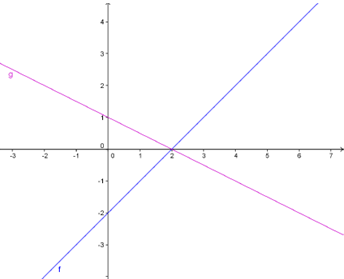
\includegraphics[width=0.7\linewidth]{Anexos-03/Imagen3}
\end{figure}

\begin{enumerate}[a.]
	\item Establezcan el conjunto de valores de $x$ para los cuales la función $h(x)$ es positiva, negativa o cero.
	\item Propongan un gráfico aproximado de $h(x)$.
\end{enumerate}
\end{problema}

\subsection{Primeras dos horas sincrónicas}\label{subsec:primeras-dos}

El desarrollo del encuentro pasara por tres momentos:

\begin{itemize}[ ]
	\item Momento 1: Socialización de las actividades previas (Problema \ref{prob:1}, \ref{prob:2}, \ref{prob:3})
	\item Momento 2: Resolución de actividades (Problema \ref{prob:4}).
	\item Momento 3: Puesta en común del problema de la clase sincrónica. Lineamientos para las actividades asincrónicas. 
\end{itemize}

\begin{problema}\label{prob:4}
Para trabajar con GeoGebra:

\begin{itemize}[-]
	\item Escriban las fórmulas que correspondan a las funciones $f(x)$ y $g(x)$ del problema 2.
	\item Usen el software para graficarlas. Introduzcan la función producto $h(x)$ como objeto dependiente. Para ello escriban en “\textit{Entrada}”: $h(x)=f(x)*g(x)$
	\begin{enumerate}[a.]
		\item Hallen, si es posible, una recta paralela al gráfico de $f$, de manera tal que al “multiplicarla” por $g$, la parábola “producto” no atraviese al eje de las $x$. Expliquen sus respuestas.
	\end{enumerate}
\end{itemize}
\end{problema}

\subsection{Primeras dos horas entre clases}\label{subsec:primeras-dos-EC}

Se habilitara en el espacio de la plataforma destinado para el taller lo siguiente:

\paragraph{Actividad del taller:}

Les pedimos que armen un escrito con la resolución del problema \ref{prob:5} posible de ser compartido en el sincrónico.

\begin{problema}\label{prob:5}

\begin{enumerate}[a.]
	\item  Propongan, si es posible, dos funciones lineales cuyo producto sea una función cuadrática que tenga mínimo y otras dos para que la función cuadrática tenga máximo. Si no hay, justifiquen la respuesta.
	\item Busquen pares de rectas para que el mínimo de la parábola “producto” esté en el primero, en el segundo, en el tercero y en el cuarto cuadrante. Si no hay, justifiquen la respuesta.
	\item Hagan lo mismo con el máximo.
\end{enumerate}
\end{problema}

\subsection{Segundas dos horas sincrónicas}\label{subsec:segundas-dos}

Comenzaremos retomando las consignas del problema \ref{prob:5} para poner en discusión. Luego se presentará las siguientes consignas:

\paragraph{Actividad del taller:}

Considerando las consignas del problema \ref{prob:6}:

\begin{itemize}[-]
	\item Anticipen posibles respuestas de los chicos y las chicas. ¿Qué ideas son necesarias tener disponible para poder responder cada pregunta? 
	\item Identifiquen en qué problemas de los trabajados previamente fueron abordadas dichas ideas.
\end{itemize}

\begin{problema}\label{prob:6}

\begin{enumerate}[1.]
	\item ¿Es cierto que siempre que “multiplicamos” dos rectas obtenemos una parábola?
	\item ¿Cómo obtenemos los ceros, el conjunto de positividad y el conjunto de negatividad de la parábola a partir de los gráficos de las rectas?
	\item ¿Es cierto que toda parábola puede ser escrita como el “producto” de dos rectas?
	\item ¿Cómo deben ser las rectas para que su “producto” sea una parábola que tenga máximo? ¿Y mínimo?
	\item ¿Cómo deben ser las rectas para que su “producto” sea una parábola con un cero doble? ¿Y con dos ceros simples?
\end{enumerate}
\end{problema}

Luego se realizará en una pizarra digital las conclusiones del problema \ref{prob:6}.

\subsection{Segundas dos horas Entre Clases}\label{subsec:segundas-dos-EC}

\paragraph{Actividad del taller:}

En el espacio del aula A partir del problema \ref{prob:8}:

\begin{itemize}
	\item Pensar en posibles resoluciones para los ítems a, b y c. ¿Qué estrategias se podrían recuperar de lo trabajado en los primeros problemas de esta secuencia? 
	\item ¿Qué argumentos podrían esbozar los alumnos y las alumnas, antes de graficar, para descartar que el gráfico, pedido en el ítem d, no será una parábola?
	\item Les pedimos que armen un escrito con sus respuestas a esta actividad ya que será un potente insumo para el análisis de los siguientes problemas.
\end{itemize}

\begin{problema}\label{prob:8}
Para hacer con lápiz y papel sin usar la computadora:

A continuación se dan los gráficos de $f(x)$ y de $g(x)$. (Figura \ref{fig:imagen4}).

\begin{figure}[h]
	\centering
	\caption{}
	\label{fig:imagen4}
	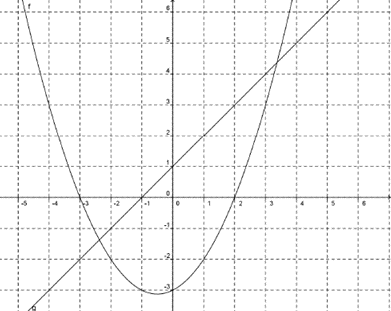
\includegraphics[width=0.6\linewidth]{Anexos-03/Imagen4}
\end{figure}

\begin{enumerate}[a.]
	\item Calcular:
	\begin{multicols}{3}
		\begin{enumerate}[i.]
		\item $h(1)=$
		\item $h(0)=$
		\item $h(-3)=$
		\item $h(-2)=$
		\item $h(3)=$
		\item $h(-4)=$
		\end{enumerate}
	\end{multicols}
	
	\item Decidir si h es positiva, negativa o cero en cada caso:
	\begin{multicols}{3}
		\begin{enumerate}[i.]
			\item $h(6)$
			\item $h(1.5)$
			\item $h(-4)$
			\item $h(0)$
			\item $h(-2.5)$
			\item $h(-20)$
		\end{enumerate}
	\end{multicols}
	
	\item Indicar ceros, el conjunto de positividad y el de negatividad.
	
	\item Graficar aproximadamente.
\end{enumerate}
\end{problema}

\subsection{Terceras dos horas sincrónicas}\label{terceras-dos}

\begin{problema}\label{prob:9}
	Con GeoGebra:
	
	\begin{enumerate}[a.]
		\item Grafiquen la recta y la parábola del problema \ref{prob:8} buscando la fórmula de ambas y grafiquen la función producto $h$. Guarden este archivo.\label{itema}
		\item El enunciado de este ítem es para dar oralmente en la clase una vez concluida la parte \ref{itema}. En un nuevo archivo vuelvan a graficar $h(x)$. ¿Pueden expresar $h$ como producto de tres rectas? En caso de ser posible, escriban la fórmula de las tres rectas que encontraron y grafiquen la función producto en la misma ventana para ver si se superpone con el gráfico de $h$. En caso de no ser posible, justifiquen por qué. Guarden este archivo.\label{itemb}
		\item Abran el archivo que guardaron en \ref{itema}. Dejen fija la parábola y muevan la recta paralelamente a ella misma, de tal manera que el producto $h$ atraviese el eje $x$ una sola vez. Guarden este archivo sin modificar el anterior (ir a “\textit{Guardar como}”).\label{itemc}
		\item Abran el archivo que guardaron en \ref{itema}. Dejen la recta fija y cambien la fórmula de la parábola para lograr que $h$ tenga un cero simple y otro doble. Guarden este archivo sin modificar el anterior.\label{itemd}
	\end{enumerate}
\end{problema}

\paragraph{Consigna de trabajo del encuentro:}

\begin{itemize}[-]
	\item Para el ítem \ref{itemb} anticipen diferentes formas de resolver analizando qué rol cumple el trabajo con los gráficos o las fórmulas en cada estrategia que propongan.
	
	\item Para los ítems \ref{itemc} y \ref{itemd}, analicen ¿Qué conocimientos o conclusiones se pueden pensar como asuntos importantes para discutir en el aula?
\end{itemize}

\subsection{Evaluación final}

La evaluación del taller consistirá en la presentación del último problema de la secuencia que podrá ser desarrollada de forma individual o grupal.

\begin{problema}\label{prob:10}
En cada caso, hallen, si existe, la fórmula de una función cúbica $h$ que verifique lo pedido. Si les parece que no existe expliquen por qué:
\begin{enumerate}[a.]
	\item Las raíces son $-5$, $-2$ y $4$, y $h$ toma valores negativos para $x$ mayores que $4$.
	\item Las raíces son $-3$, $2$ y $8$, y el gráfico de $h$ corta al eje de las $y$ en $12$.
	\item Las raíces son solamente $2$ y $7$.
	\item Las raíces son solamente cero y $-1$, y $h(1) = 10$.
	\item La función que encontraron en cada caso, ¿es la única que cumple esas condiciones? Si creen que sí, justifiquen; y si creen que no, hallen al menos tres fórmulas diferentes.
\end{enumerate}
\end{problema}

\paragraph{Consigna del taller para el problema \ref{prob:10}, estudien:}
\begin{itemize}
	\item ¿Qué trabajo sobre el registro algebraico y/o sobre el registro gráfico podría estar presente en las resoluciones del ítem a y del b?
	\item ¿Qué argumentos podrían dar los y las estudiantes en los casos donde no se puede obtener la función pedida?
	\item ¿Cómo imaginan una validación para cada caso, posible de realizar en el aula del secundario?
\end{itemize}

Este trabajo es para entregar en un archivo de Word, en letra Times New Roman, tamaño 12, indicando dentro del mismo el nombre del taller, junto con los y las integrantes del grupo y la consigna del trabajo. Luego, el desarrollo de la misma.

\section{Bibliografía}

\nocite{introduccion-polinomios,conf-llanos-v,llanos-v}
\printbibliography

\end{document}